\subsection{图的存储及基本操作}\qanswerloc{216}

\begin{qitems}
    \begin{bbox}
        \qitem 已知带权有向图 $G$ 的邻接矩阵如下图所示,请画出该带权有向图 $G$。
        \[
            \begin{pmatrix}
                0 & 15 & 2 & 12 & \infty & \infty & \infty \\
                \infty & 0 & \infty & \infty & 6 & \infty & \infty \\
                \infty & \infty & 0 & \infty & 8 & 4 & \infty \\
                \infty & \infty & \infty & 0 & \infty & \infty & 3 \\
                \infty & \infty & \infty & \infty & 0 & \infty & 9 \\
                \infty & \infty & 5 & \infty & \infty & 0 & 10 \\
                \infty & 4 & \infty & \infty & \infty & \infty & 0
            \end{pmatrix}
        \]
    \end{bbox}

    \begin{solution}
        该带权有向图如下图所示:
        \begin{center}
            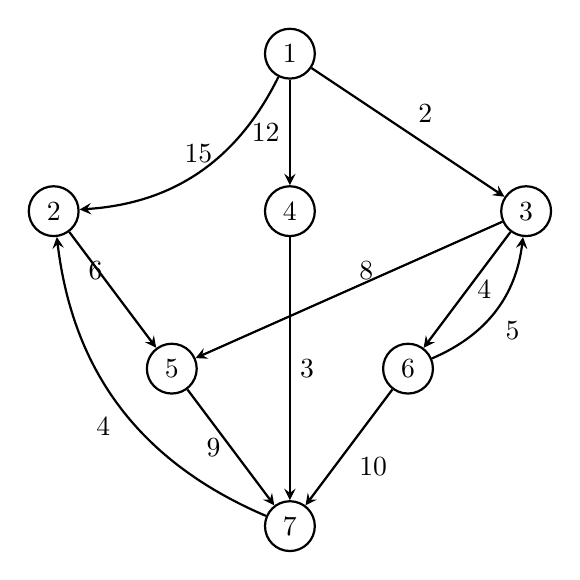
\begin{tikzpicture}[->, >=stealth, auto, node distance=2.5cm, thick]
                \tikzstyle{vertex}=[circle, draw, minimum size=18pt, inner sep=2pt]
                
                \node[vertex] (v1) at (0, 4) {1};
                \node[vertex] (v2) at (-3, 2) {2};
                \node[vertex] (v3) at (3, 2) {3};
                \node[vertex] (v4) at (0, 2) {4};
                \node[vertex] (v5) at (-1.5, 0) {5};
                \node[vertex] (v6) at (1.5, 0) {6};
                \node[vertex] (v7) at (0, -2) {7};
                
                \path (v1) edge[bend left] node[pos=0.5, above] {15} (v2);
                \path (v1) edge node[pos=0.5, above right] {2} (v3);
                \path (v1) edge node[pos=0.5, left] {12} (v4);
                \path (v2) edge node[pos=0.5, above left] {6} (v5);
                \path (v3) edge node[pos=0.5, above right] {8} (v5);
                \path (v3) edge node[pos=0.5, right] {4} (v6);
                \path (v4) edge node[pos=0.5, right] {3} (v7);
                \path (v5) edge node[pos=0.5, left] {9} (v7);
                \path (v6) edge[bend right] node[pos=0.5, below right] {5} (v3);
                \path (v6) edge node[pos=0.5, below right] {10} (v7);
                \path (v7) edge[bend left] node[pos=0.5, below left] {4} (v2);
            \end{tikzpicture}
        \end{center}
    \end{solution}

    \begin{bbox}
        \qitem 设图 $G = (V, E)$ 以邻接表存储,如下图所示。画出其邻接矩阵存储及图 $G$。
        \imgin[0.7]{}{fig/fig6.2.2.png}
    \end{bbox}

    \begin{solution}
        根据邻接表,该图是无向图,其邻接矩阵为:
        \[
            \begin{pmatrix}
                0 & 1 & 1 & 1 & 0 \\
                1 & 0 & 1 & 1 & 1 \\
                1 & 1 & 0 & 1 & 0 \\
                1 & 1 & 1 & 0 & 1 \\
                0 & 1 & 0 & 1 & 0
            \end{pmatrix}
        \]
        图 $G$ 如下图所示:
        \begin{center}
            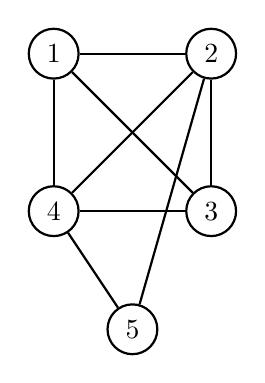
\begin{tikzpicture}[-, auto, node distance=2cm, thick]
                \tikzstyle{vertex}=[circle, draw, minimum size=18pt, inner sep=2pt]
                
                \node[vertex] (v1) at (0, 2) {1};
                \node[vertex] (v2) at (2, 2) {2};
                \node[vertex] (v3) at (2, 0) {3};
                \node[vertex] (v4) at (0, 0) {4};
                \node[vertex] (v5) at (1, -1.5) {5};
                
                \path (v1) edge (v2);
                \path (v1) edge (v3);
                \path (v1) edge (v4);
                \path (v2) edge (v3);
                \path (v2) edge (v4);
                \path (v2) edge (v5);
                \path (v3) edge (v4);
                \path (v4) edge (v5);
            \end{tikzpicture}
        \end{center}
    \end{solution}

    \begin{bbox}
        \qitem 对 $n$ 个顶点的无向图和有向图,分别采用邻接矩阵和邻接表表示时,试问:
        \begin{subqitems}
            \subqitem 如何判别图中有多少条边?
            \subqitem 如何判别任意两个顶点 $i$ 和 $j$ 是否有边相连?
            \subqitem 任意一个顶点的度是多少?
        \end{subqitems}
    \end{bbox}

    \begin{bbox}
        \qitem 如何对无环有向图中的顶点重新编号,使得该图的邻接矩阵中所有的 1 都集中到对角线以上?
    \end{bbox}

    \begin{bbox}
        \qitem 写出从图的邻接表表示转换成邻接矩阵表示的算法。
    \end{bbox}

    \begin{bbox}
        \qitem 【2015统考真题】已知有5个顶点的图G如下图所示。
        \imgin[0.6]{}{fig/fig6.2.6.png}
        \begin{subqitems}
            \subqitem 写出图G的邻接矩阵A(行、列下标从0开始)。
            \subqitem 求$A^2$,矩阵$A^2$中位于0行3列元素值的含义是什么?
            \subqitem 若已知具有n($n \ge 2$)个顶点的图的邻接矩阵为B,则$B^m$($2 \le m \le n$)中非零元素的含义是什么?
        \end{subqitems}
    \end{bbox}

    \begin{bbox}
        \qitem 【2021统考真题】已知无向连通图 $G$ 顶点集为 $V$ 和边集 $E$ 组成,$|E|>0$。当 $G$ 中度为奇数的顶点个数为不大于2的偶数时,G 存在包含所有边且长度为 $|E|$ 的路径(称为 EL 路径)。设图 $G$ 采用邻接矩阵存储,类型定义如下:
        \begin{lstlisting}[language=C, basicstyle=\ttfamily\small]
typedef struct {
    int numVertices, numEdges;  //图中实际的顶点数和边数
    char VerticesList[MAXV];    //顶点表, MAXV为已定义常量
    int Edge[MAXV][MAXV];       //邻接矩阵
} MGraph;
        \end{lstlisting}
        请设计算法 \lstinline{int IsExistEL(MGraph G)},判断 G 是否存在 EL 路径,若存在,则返回1,否则返回0。要求:
        \begin{subqitems}
            \subqitem 给出算法的基本设计思想。
            \subqitem 根据设计思想,采用C或C++语言描述算法,关键之处给出注释。
            \subqitem 说明你所设计算法的时间和空间复杂度。
        \end{subqitems}
    \end{bbox}
 
    \begin{bbox}
            \qitem 【2023统考真题】已知有向图G采用邻接矩阵存储,类型定义如下:
            \begin{lstlisting}[language=C, basicstyle=\ttfamily\small]
typedef struct {
    int numVertices, numEdges;  //图的顶点数和有向边数
    char VerticesList[MAXV];    //顶点表, MAXV为已定义常量
    int Edge[MAXV][MAXV];       //邻接矩阵
} MGraph;
            \end{lstlisting}
            将图中出度大于入度的顶点称为K顶点。例如,在下图中,顶点a和b为K顶点。
            \imgin[0.6]{}{fig/fig6.2.8.png}

            请设计算法 \lstinline{int printVertices(MGraph G)},对给定的任意非空有向图G,输出G中所有的K顶点,并返回K顶点的个数。要求:
            \begin{subqitems}
                \subqitem 给出算法的基本设计思想。
                \subqitem 根据设计思想,采用C或C++语言描述算法,关键之处给出注释。
            \end{subqitems}
    \end{bbox}
    
\end{qitems} 